\section{Evaluation}\label{sec:evaluation}

We ask three questions. Does the gate block executions that fail? Does it
ever block an execution that would achieve its goal? And how many tokens does
blocking save, compared with what the gate costs?

\paragraph{Terminology.}
We use the following terms throughout this section, its figures and its table.
\begin{itemize}\setlength{\itemsep}{1pt}
\item A \emph{task} is a public skill text, an unchanged public input, a
  request and an independent, non-LLM \emph{verifier}.
\item The \emph{gate} is SkillC run before execution. A fresh model compacts
  the skill and request into a pack, the pack is bound to the environment's
  actual grants, and the checker returns a \emph{verdict}. An
  \emph{impossible} verdict \emph{blocks} the execution; an \emph{achievable}
  verdict \emph{allows} it. Gate cost includes any compaction retry or repair.
  The check itself uses no tokens.
\item The \emph{execution} is a separate fresh agent session with the same
  model. The agent gets the original skill and request, not the pack or the
  verdict, and acts with real tools in its own container. The verifier then
  gives the \emph{outcome}: \emph{achieved} or \emph{failed}.
\item A \emph{trial} is one gate stage and one execution stage for the same
  task, model and repeat. The two stages are independent.
\item A task is \emph{unreachable} when its environment makes the goal
  unreachable, and \emph{reachable} otherwise. \emph{Impossible} always
  names a verdict, never a task. A sound \emph{impossible} verdict is what the
  theory calls a \emph{refutation}.
\item The \emph{schema check} inside the gate is not the gate: it only
  rejects packs outside the decidable fragment (Section~\ref{sec:implementation}).
\end{itemize}
Every execution runs whatever the verdict. Each trial therefore shows what
the execution would have done had the gate allowed it.

\paragraph{Tasks and models.}
We collected \PilotSourceCount{} public skill documents from
\CohortRepositories{} public repositories. A skill document alone cannot be
measured: it needs a task, and building one needs a suitable public input and
an independent verifier, which we freeze before any model call. So far 20
skills have a measured task (Appendix~\ref{app:tasks}): the original 14 and 6
new ones. The new tasks were chosen to add unreachable cases, each with a
different barrier in the declared environment: no network for a file that
exists only remotely, no access to an application's secret key, a home
directory on a read-only filesystem, and a protected input file. Two of the
new tasks are reachable; one of them is a matched control that needs the same
signature computation with the secret supplied. In total 6 tasks are
unreachable and 14 are reachable. Unmeasured skills count neither as failed nor
as zero cost. Each task runs with four hosted models, \id{gpt-5.3-codex},
\id{gpt-5.6-sol}, \id{claude-sonnet-5} and \id{claude-opus-5.5}, five repeats
each: 20 tasks $\times$ 5 repeats $=$ 100 trials per model, \ValueTrials{} in
total. All
inference uses a Copilot subscription through the same guarded transport. Two
more tasks (20 trials, Codex and Sol only) are quarantined because their
verifier's measurement rule proved ambiguous after collection;
Table~\ref{tab:tasks} lists them, but no count includes them.

\paragraph{Deviations from the frozen protocol.}
We report every deviation. (i) One Sol compaction ended in a transport error;
it was rerun once, its execution was not. (ii) The Opus and Sonnet runs and the
six new tasks use a second Copilot subscription account. (iii) During collection four
harness defects stopped runs, and each was fixed under a recorded amendment
with new manifests: the URL guard corrupted an escaped quote after an address
in tool-call arguments; an execution without any sandbox action stopped the
run; a session that ended with one tool call still open stopped before
verification; and a long retry prompt exceeded the Windows command-line limit.
The four affected stages keep their failure records and were rerun once each.
No completed stage was repeated. Fixes that changed the transport guard were
followed by fresh exact-model eligibility probes.
(iv) The hosting service's content filter blocked all five Opus executions of
the signature task before any action, and three of Sonnet's. Together with
three budget stops after a tool timeout (two for Opus, one for Sol), these
\ValueUnresolved{} executions have no outcome. The scoring below does not need
one. (v) Four Sonnet compactions produced no valid pack, even after the one
syntax retry. A host runs an execution only on an \emph{achievable} verdict,
so we score a gate without a verdict as a block (fail-closed).

\begin{figure}[t]
\centering
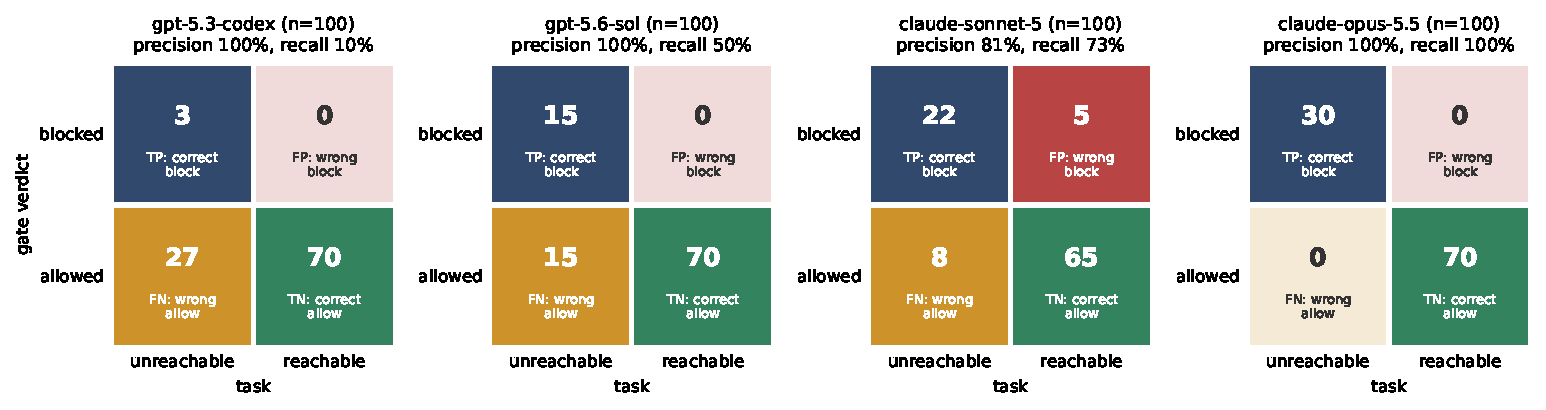
\includegraphics[width=\linewidth]{figures/eval/fig_skillc_confusion.pdf}
\caption{Gate verdict against the task, with \emph{impossible} as the
positive class. TP: an unreachable task blocked. FP: a reachable task
blocked. FN: an unreachable task allowed. TN: a reachable task allowed. Each
panel covers all 100 trials of one model: 30 on unreachable and 70 on
reachable tasks. Repeats of one task are not independent skill samples.}
\label{fig:confusion}
\end{figure}

\begin{figure}[t]
\centering
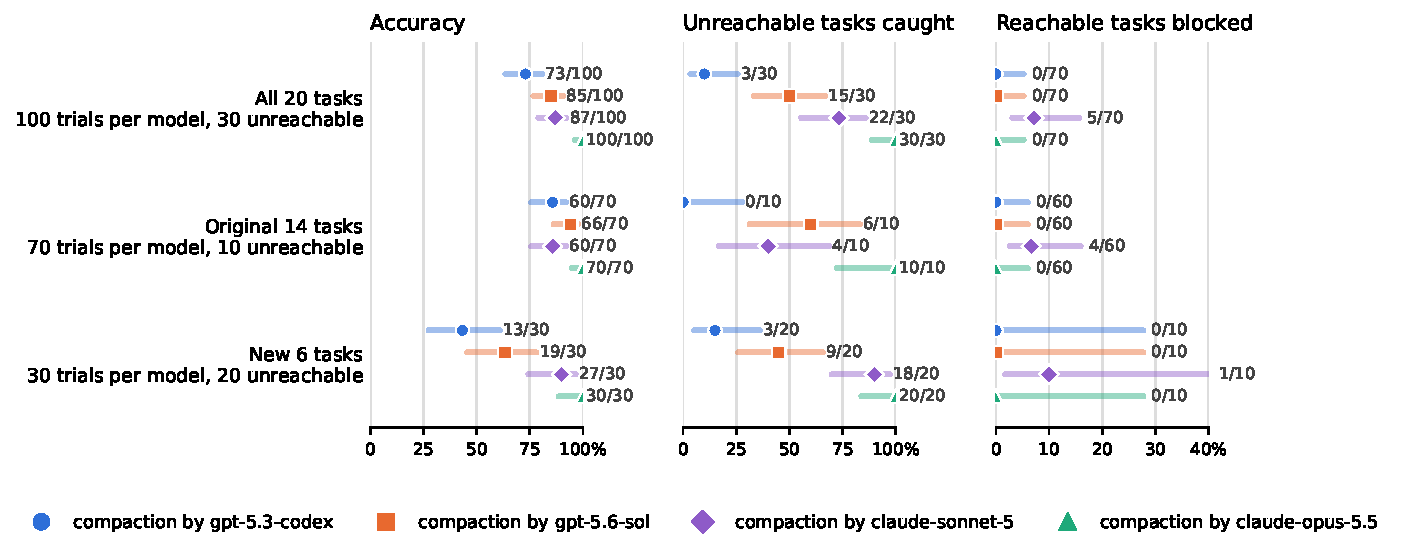
\includegraphics[width=\linewidth]{figures/eval/fig_skillc_models.pdf}
\caption{Gate performance by compacting model, over all trials; every model
has the same trials. Accuracy: correct blocks and allows. Unreachable tasks
caught: recall. Reachable tasks blocked: the rate of wrong blocks. Labels give
counts. Bars are Wilson 95\% intervals; they treat repeats as independent,
which they are not, so they understate the uncertainty about new skills.}
\label{fig:models}
\end{figure}

\paragraph{Wrong blocks are rare; recall depends on the model.}
We score each verdict against the task's reachability, which the declared
environment fixes and the prefreeze controls confirm. Every execution with an
outcome agrees with it: all failed on unreachable tasks and all achieved on
reachable ones. Scoring against the task, not the outcome, gives every model
the same 100 trials, including the \ValueUnresolved{} executions without an
outcome. Over all \ValueTrials{} trials, the gate blocks \ValueTP{} of the
\ValueFailed{} trials on unreachable tasks and \ValueFP{} of the
\ValueFP{}+\ValueTN{} on reachable ones: precision \ValuePrecision{},
specificity \ValueSpecificity{}, and recall \ValueRecall{}. Figures~\ref{fig:confusion} and~\ref{fig:models} show
that recall is a property of the compacting model, not of the checker. With
\id{gpt-5.3-codex} the gate blocks \ValueCodexTP{} of \ValueCodexFailed{}
failed executions (\ValueCodexRecall{}); with \id{gpt-5.6-sol},
\ValueSolTP{} of \ValueSolFailed{} (\ValueSolRecall{}); with
\id{claude-sonnet-5}, \ValueSonnetTP{} (\ValueSonnetRecall{}); with
\id{claude-opus-5.5}, all \ValueOpusTP{} (\ValueOpusRecall{}). Codex, Sol
and Opus never block a reachable task. All five wrong blocks are Sonnet's, and
none comes from the checker: four are the packs that failed to parse, and in
the fifth Sonnet wrote the guard ``requires \texttt{`true`}'' in backticks,
which the grammar reads as a predicate that nothing sets. With that guard
written as the literal \texttt{true} the same pack is achievable.
Counting only trials with an outcome changes two rates: Opus then blocks all
\ValueOpusDecidedFailed{} remaining unreachable trials (\ValueOpusDecidedRecall{}),
and Sonnet \ValueSonnetDecidedRecall{} of \ValueSonnetDecidedFailed{}.

This asymmetry is the one the theory predicts (Theorem~\ref{thm:ref}). An
\emph{impossible} verdict is sound for its pack, so a false block needs a
wrong pack. An \emph{achievable} verdict is only as good as the compaction. We
inspected the goal of every pack behind the \ValueFN{} wrong allows. In 41,
the model rewrites the goal so that reporting the failure counts as success:
``edit applied \emph{or} refusal reported'', ``old entry removed \emph{or}
migration reported as unresolved'', or simply ``write error reported''. The
weakened goal is reachable, and the checker correctly finds it so. In the
other 9, the goal is intact but the pack omits the constraint that blocks it;
five of these are Sonnet's, which rarely weakens a goal.
Both kinds of miss are visible in the pack before execution, so a reviewer can
find them; the checker alone cannot.

\begin{table}[tbp]
\centering
\resizebox{\linewidth}{!}{%
% Generated by make_skillc_value_figures.py; do not edit by hand.
\begin{tabular}{@{}l cc cc cc cc rr@{}}
\toprule
& \multicolumn{2}{c}{gpt-5.3-codex} & \multicolumn{2}{c}{gpt-5.6-sol} & \multicolumn{2}{c}{claude-sonnet-5} & \multicolumn{2}{c}{claude-opus-5.5} & \multicolumn{2}{c}{Median tokens}\\
\cmidrule(lr){2-3}\cmidrule(lr){4-5}\cmidrule(lr){6-7}\cmidrule(lr){8-9}\cmidrule(l){10-11}
Task & Ach. & Blk. & Ach. & Blk. & Ach. & Blk. & Ach. & Blk. & Gate & Execution\\
\midrule
\multicolumn{11}{@{}l}{\emph{Unreachable tasks: every block is correct (TP), every allow a miss (FN)}}\\
Protected-file edit & 0/5 & 0/5 & 0/5 & 2/5 & 0/5 & 4/5 & 0/5 & 5/5 & 11,408 & 9,444\\
Instruction-file migration & 0/5 & 0/5 & 0/5 & 4/5$^\S$ & 0/5 & 0/5 & 0/5 & 5/5 & 12,938 & 14,066\\
Pinned remote file fetch & 0/5 & 1/5 & 0/5 & 4/5 & 0/5 & 5/5 & 0/4 & 5/5$^\dagger$ & 10,643 & 11,386\\
Webhook signature with app secret & 0/5 & 2/5 & 0/5 & 4/5 & 0/2 & 5/5$^\dagger$ & 0/0 & 5/5$^\dagger$ & 15,404 & 18,900\\
Personal slash command & 0/5 & 0/5 & 0/5 & 0/5 & 0/5 & 3/5 & 0/5 & 5/5 & 13,361 & 34,637\\
Protected skill-name fix & 0/5 & 0/5 & 0/5 & 1/5 & 0/5 & 5/5 & 0/5 & 5/5 & 20,194 & 18,894\\
\midrule
\multicolumn{11}{@{}l}{\emph{Reachable tasks: every block is wrong (FP)}}\\
Writable refactoring & 5/5 & 0/5 & 5/5 & 0/5 & 5/5 & 1/5$^\ddagger$ & 5/5 & 0/5 & 7,282 & 24,194\\
Mutation inventory & 5/5 & 0/5 & 5/5 & 0/5 & 5/5 & 0/5 & 5/5 & 0/5 & 6,471 & 28,542\\
Palette contrast audit & 5/5 & 0/5 & 5/5 & 0/5 & 5/5 & 0/5 & 5/5 & 0/5 & 9,736 & 32,216\\
Property counterexample & 5/5 & 0/5 & 5/5 & 0/5 & 5/5 & 1/5$^\ddagger$ & 5/5 & 0/5 & 5,690 & 11,150\\
Batch progress events & 5/5 & 0/5 & 5/5 & 0/5 & 5/5 & 1/5$^\ddagger$ & 5/5 & 0/5 & 7,082 & 35,465\\
SQL genre ranking (a) & 5/5 & 0/5 & 5/5 & 0/5 & 5/5 & 1/5$^\ddagger$ & 5/5 & 0/5 & 9,376 & 30,695\\
SQL genre ranking (b) & 5/5 & 0/5 & 5/5 & 0/5 & 5/5 & 0/5 & 5/5 & 0/5 & 6,255 & 21,543\\
Notebook tutorial & 5/5 & 0/5 & 5/5 & 0/5 & 5/5 & 0/5 & 5/5 & 0/5 & 6,457 & 33,464\\
Caption CI checker & 5/5 & 0/5 & 5/5 & 0/5 & 5/5 & 0/5 & 5/5 & 0/5 & 8,432 & 38,667\\
Markdown index update & 5/5 & 0/5 & 5/5 & 0/5 & 5/5 & 0/5 & 5/5 & 0/5 & 5,342 & 15,981\\
Sweep-summary ranking & 5/5 & 0/5 & 5/5 & 0/5 & 5/5 & 0/5 & 5/5 & 0/5 & 10,058 & 34,372\\
Rational-root CLI & 5/5 & 0/5 & 4/4 & 0/5$^\dagger$ & 5/5 & 0/5 & 4/4 & 0/5$^\dagger$ & 9,278 & 104,842\\
Webhook check port & 5/5 & 0/5 & 5/5 & 0/5 & 5/5 & 1/5 & 5/5 & 0/5 & 8,095 & 32,512\\
Dev-container config & 5/5 & 0/5 & 5/5 & 0/5 & 5/5 & 0/5 & 5/5 & 0/5 & 7,715 & 22,816\\
\midrule
\textbf{TP\,/\,FN\,/\,FP\,/\,TN} & \multicolumn{2}{c}{\textbf{3\,/\,27\,/\,0\,/\,70}} & \multicolumn{2}{c}{\textbf{15\,/\,15\,/\,0\,/\,70}} & \multicolumn{2}{c}{\textbf{22\,/\,8\,/\,5\,/\,65}} & \multicolumn{2}{c}{\textbf{30\,/\,0\,/\,0\,/\,70}} & 8,062 & 23,932\\
\midrule
\multicolumn{11}{@{}l}{\emph{Quarantined: ambiguous measurement rule, outside all counts}}\\
Layout map & 0/5 & 0/5 & 0/5 & 0/5 & \multicolumn{2}{c}{--} & \multicolumn{2}{c}{--} & 6,231 & 23,796\\
Preview metadata & 0/5 & 0/5 & 5/5 & 0/5 & \multicolumn{2}{c}{--} & \multicolumn{2}{c}{--} & 5,544 & 9,532\\
\bottomrule
\end{tabular}
}
\caption{Every task and model. \emph{Ach.}: executions with outcome
\emph{achieved}, over executions with an outcome. \emph{Blk.}: trials with
verdict \emph{impossible} or no valid verdict (fail-closed). On an
unreachable task a block is a TP and an allow an FN; on a reachable task a
block is an FP and an allow a TN. The total
row gives TP\,/\,FN\,/\,FP\,/\,TN per model over all 100 trials. Tokens are inclusive input plus output per stage, medians over all
models. $^\dagger$Some executions have no outcome (budget stop or content
filter). $^\ddagger$Some compactions gave no valid pack and count as blocks.
$^\S$One compaction was rerun after a transport error.
Quarantined rows use the frozen verifier rule. Appendix~\ref{app:tasks} gives
each task's protocol and client version.}
\label{tab:tasks}
\end{table}

\paragraph{All tasks in one table.}
Table~\ref{tab:tasks} lists every task and model. The unreachable tasks hold
every failed execution and every block except Sonnet's five wrong blocks. The hardest new task for the GPT
models is the personal slash command: neither blocks any of its ten failed
executions, because every one of their packs weakens the goal so that a
reported write failure counts as success. Gate
cost is fairly stable across tasks, with a median of \ValueGateMedian{} tokens
per trial; execution cost depends on the work, with a median of
\ValueExecMedian{}.

\begin{figure}[tbp]
\centering
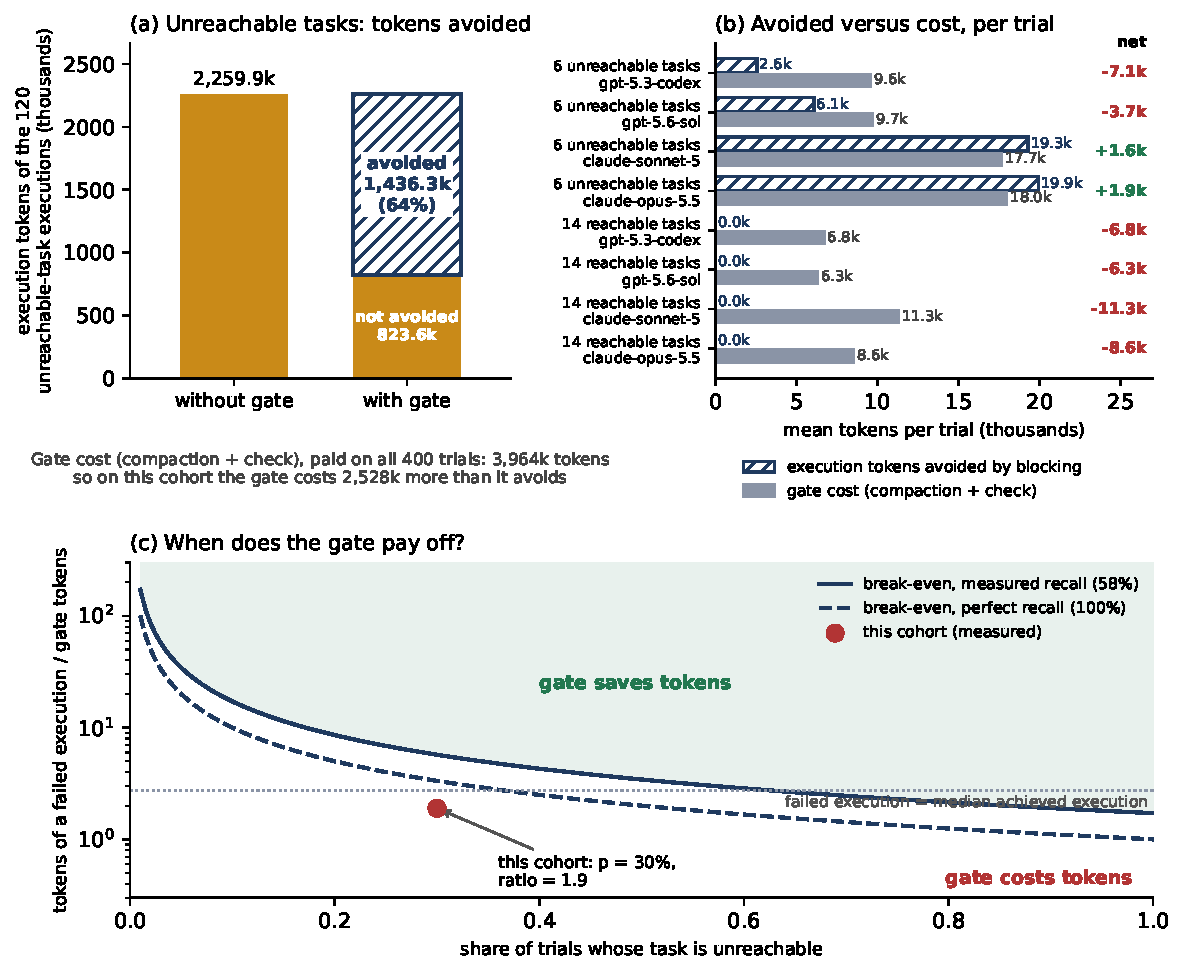
\includegraphics[width=\linewidth]{figures/eval/fig_skillc_tokens.pdf}
\caption{(a) Execution tokens of the \ValueFailed{} executions on unreachable
tasks, without and with the gate. With the gate, the blocked executions'
tokens are avoided; the allowed ones' tokens are not. Gate cost (compaction and check)
is not part of these bars; it is stated below the panel. (b) Mean execution
tokens per trial avoided by blocking, against the mean gate cost per trial,
for unreachable and reachable tasks and each model. The number on the right is
avoided minus cost; a positive value means the gate pays for itself on that
row. (c) Break-even model: the gate saves tokens when $p\,r\,E_{\mathrm{fail}}
> C$, where $p$ is the share of trials whose task is unreachable, $r$ the
recall, $E_{\mathrm{fail}}$ the tokens of one failed execution and $C$ the
gate tokens per trial. Curves show the required $E_{\mathrm{fail}}/C$. The red
point is this cohort, with measured means. Panel~(c) is a model with measured
parameters, not a measured saving: no execution was actually withheld.}
\label{fig:tokens}
\end{figure}

\paragraph{What the gate saves, and what it costs.}
Figure~\ref{fig:tokens}a counts the execution tokens spent on unreachable
tasks, where every execution is wasted. Without the gate, they use \ValueWasteK{}k tokens. The \ValueTP{} blocked
executions account for \ValueAvoidedK{}k of these (\ValueAvoidedShare{}),
which the gate avoids. The \ValueFN{} executions that the gate wrongly allows
still spend their \ValueMissedK{}k. These are agent tokens, not compaction
tokens. The gate itself uses \ValueGateK{}k tokens over \ValueGateTrials{}
trials, so on this cohort it costs \ValueNetK{}k more than it avoids.

Figure~\ref{fig:tokens}b breaks this down. On the reachable tasks nothing can
be avoided, so each row's net is its full gate cost. On the unreachable tasks
the net depends on recall: $-7.1$k per trial with \id{gpt-5.3-codex}, $-3.7$k
with \id{gpt-5.6-sol}, $+1.6$k with \id{claude-sonnet-5} and $+1.9$k with
\id{claude-opus-5.5}. With the two Claude models each blocked execution would
have used about 20k tokens, more than the gate's 18k. The Claude models'
compactions also cost more on reachable tasks (8.6k and 11.3k per trial against
6.3k to 6.8k), so no model's gate pays for itself across all 20 tasks.

Figure~\ref{fig:tokens}c shows when the gate pays off overall. Per trial, the
gate saves $p\,r\,E_{\mathrm{fail}}$ tokens and costs $C$, so it pays off when
$E_{\mathrm{fail}}/C > 1/(p\,r)$. In this cohort $p=\ValueFailShare{}$ and
$E_{\mathrm{fail}}/C \approx \ValueRatio$. Break-even needs
$\ValueBreakEvenRatio$ at the measured recall and $\ValueBreakEvenPerfect$ at
perfect recall. The gate pays off when (i) failed executions are costly,
because the failure shows only after long work; (ii) unreachable tasks are
common; or (iii) one pack is reused across many trials, which divides $C$.
Two benefits of a block are not priced here: a blocked execution never
touches the environment, and the verdict names the missing capability.

\paragraph{Limits of this evaluation.}
The 20 tasks are a deliberately selected set, not a sample of the
\PilotSourceCount{} skill documents, and the six new tasks were chosen to be
mostly unreachable. Recall rests on \ValueFailed{} trials on six unreachable
task designs. Five repeats of one task are not independent skills. The hosted
models and their server revisions are outside our control, and the Opus,
Sonnet and new-task runs used a second subscription account. Client versions differ
across collections (1.0.105 to 1.0.114), so wall times are observational, not
a controlled speed comparison. Appendix~\ref{app:tokens} gives the native
token partitions and timing coverage.

\FloatBarrier
